%%%%%%%%%%%%%%%%%%%%%%%%%%%%%%%%%%%%%%%%%
% Beamer Presentation
% LaTeX Template
% Version 1.0 (10/11/12)
%
% This template has been downloaded from:
% http://www.LaTeXTemplates.com
%
% License:
% CC BY-NC-SA 3.0 (http://creativecommons.org/licenses/by-nc-sa/3.0/)
%
%%%%%%%%%%%%%%%%%%%%%%%%%%%%%%%%%%%%%%%%%

%----------------------------------------------------------------------------------------
%	PACKAGES AND THEMES
%----------------------------------------------------------------------------------------

\documentclass{beamer}

\mode<presentation> {

% The Beamer class comes with a number of default slide themes
% which change the colors and layouts of slides. Below this is a list
% of all the themes, uncomment each in turn to see what they look like.

%\usetheme{default}
%\usetheme{AnnArbor}
%\usetheme{Antibes}
%\usetheme{Bergen}
%\usetheme{Berkeley}
%\usetheme{Berlin}
%\usetheme{Boadilla}
%\usetheme{CambridgeUS}
%\usetheme{Copenhagen}
%\usetheme{Darmstadt}
%\usetheme{Dresden}
%\usetheme{Frankfurt}
%\usetheme{Goettingen}
%\usetheme{Hannover}
%\usetheme{Ilmenau}
%\usetheme{JuanLesPins}
%\usetheme{Luebeck}
\usetheme{Madrid}
%\usetheme{Malmoe}
%\usetheme{Marburg}
%\usetheme{Montpellier}
%\usetheme{PaloAlto}
%\usetheme{Pittsburgh}
%\usetheme{Rochester}
%\usetheme{Singapore}
%\usetheme{Szeged}
%\usetheme{Warsaw}

% As well as themes, the Beamer class has a number of color themes
% for any slide theme. Uncomment each of these in turn to see how it
% changes the colors of your current slide theme.

%\usecolortheme{albatross}
%\usecolortheme{beaver}
%\usecolortheme{beetle}
%\usecolortheme{crane}
\usecolortheme{dolphin}
%\usecolortheme{dove}
%\usecolortheme{fly}
%\usecolortheme{lily}
%\usecolortheme{orchid}
%\usecolortheme{rose}
%\usecolortheme{seagull}
%\usecolortheme{seahorse}
%\usecolortheme{whale}
%\usecolortheme{wolverine}

%\setbeamertemplate{footline} % To remove the footer line in all slides uncomment this line
\setbeamertemplate{footline}[page number] % To replace the footer line in all slides with a simple slide count uncomment this line

%\setbeamertemplate{navigation symbols}{} % To remove the navigation symbols from the bottom of all slides uncomment this line
}


\usepackage{graphicx} % Allows including images
\usepackage{booktabs} % Allows the use of \toprule, \midrule and \bottomrule in tables
\usepackage[absolute,overlay]{textpos}
\usepackage{multicol}
\usepackage{pseudocode}
\usepackage[framemethod=TikZ]{mdframed}
\usepackage{graphics}
\usepackage{appendixnumberbeamer}

%\hypersetup{
%	colorlinks = true,
%	linkcolor = red
%}

%\makeatletter
%\let\@mycite\@cite
%\def\@cite#1#2{{\hypersetup{linkcolor=green!60!black}[{#1\if@tempswa , #2\fi}]}}
%\makeatother



%----------------------------------------------------------------------------------------
%	TITLE PAGE
%----------------------------------------------------------------------------------------

\title[Interring programs structure from an execution trace]
{
	\textit{Master thesis} \\
	Master in Research and Innovation \\
	\vspace{0.5cm}
	%\hrulefill \\
	\textbf{Inferring programs structure from \\
		an execution trace} \\
	%\hrulefill \\
}

\author
{%
	\texorpdfstring{
	\begin{multicols}{2}
		{\small \textit{Author}}\\
		Juan Francisco Mart\'inez Vera\\
		\columnbreak
		{\small \textit{Supervisor}}\\
		Jes\'us Labarta Mancho\\
	\end{multicols}
	}
	{ }
}
\institute[FIB, UPC]
{
	Facultat d'Inform\`atica de Barcelona (FIB) \\
	Universitat Polit\`ecnica de Catalunya (UPC)
	\begin{figure}
		
\includegraphics[width=30px]{imgs/logo_upc.png}
	\end{figure}
}
\date{\today}

\AtBeginSection[]
{
	\begin{frame}<beamer>
		\frametitle{Outline for section \thesection}
		\tableofcontents[currentsection]
	\end{frame}
}

\begin{document}
%\logo{
\includegraphics[height=0.5cm]{imgs/logo_upc.png}}

\begin{frame}
\titlepage
\end{frame}

\begin{frame}[allowframebreaks]
%\frametitle{Presentation outline}
\tableofcontents
\end{frame}

%----------------------------------------------------------------------------------------
%	PRESENTATION SLIDES
%----------------------------------------------------------------------------------------

\section{Context}
%\subsection{High Performance Computing}
%\begin{frame}
%\frametitle{High Performance Computing}
%\begin{itemize}
%	\item Becomes the third support of science with mathematics and theory
%	\item Tremendous improvement in all transformation hierarchy layers
%\end{itemize}
%\begin{figure}
%	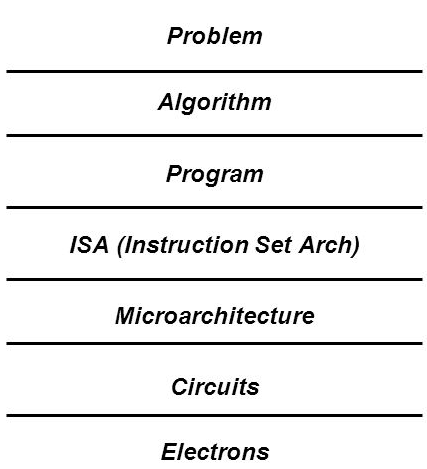
\includegraphics[width=100px]{imgs/transformationhierarchy.png}
%	\caption{Transformation hierarchy}
%\end{figure}
%\begin{textblock*}{5cm}(40px,160px) % {block width} (coords)
%	\includegraphics<+(1)->[width=70px]{imgs/moore_prediction.png}
%\end{textblock*}
%\begin{textblock*}{5cm}(40px,100px) % {block width} (coords)
%	\includegraphics<+(1)->[width=70px]{imgs/microarchitecture.png}
%\end{textblock*}
%\begin{textblock*}{5cm}(270px,170px) % {block width} (coords)
%	\includegraphics<+(1)->[width=70px]{imgs/multicore.png}
%\end{textblock*}
%\begin{textblock*}{5cm}(270px,100px) % {block width} (coords)
%	\includegraphics<+(1)->[width=70px]{imgs/program_simulation.png}
%\end{textblock*}
%\end{frame}

\subsection{Performance Analysis}
\begin{frame}
\frametitle{Performance Analysis}
\begin{itemize}
%	\item Focused on Program layer
	\item Aid to detect \textbf{bottlenecks}
	\begin{itemize}
		\item That prevents from better performance
	\end{itemize}
	\item Requires high skilled analyst...
	\item ... so developers are not used to work with them
	\begin{itemize}
		\item But derive this work to actual specialist
		\item Analyst are used to \textbf{work with codes they are not familiar with}.
		\item e.g. POP project
	\end{itemize}

	\begin{figure}
		\includegraphics[height=0.3\textheight]{imgs/meeting-peoples.png}
	\end{figure}
\end{itemize}

%\begin{multicols}{2}
%	\begin{figure}
%		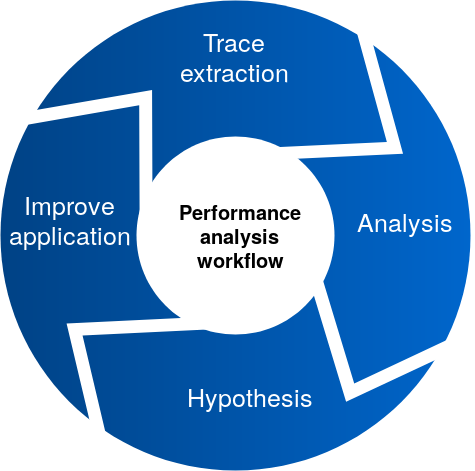
\includegraphics[height=80px]{imgs/performance_analysis_diagram.png}
%		\caption{Performance analysis workflow}
%	\end{figure}
%	\columnbreak
%
%	\begin{figure}
%		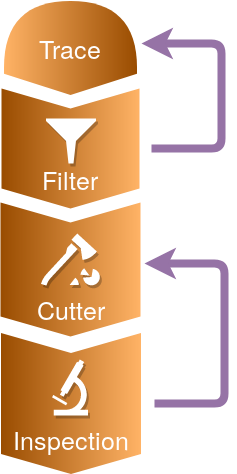
\includegraphics[height=80px]{imgs/analysis_subphases.png}
%		\caption{Analysis subphases}
%	\end{figure}
%\end{multicols}
\end{frame}

\section{Motivations}
\begin{frame}
\frametitle{Motivations}
\begin{block}{About improve understandability}
	Providing application structure will lead to better understandability about what the application is doing.
\end{block}
\pause
\begin{block}{About improve reports}
	Having the structure of the application the communication with developer can be improved
\end{block}
\end{frame}

\section{Objectives}
\begin{frame}
\frametitle{Objective}
	\begin{exampleblock}{The objective for this thesis is...}
		Find out a way to \textbf{expose the structure} of the application, by means of a post-mortem trace analysis, in order to improve the understandability of the analyst and the communication with the developers.
	\end{exampleblock}
\end{frame}

\section{State of the Art}

\begin{frame}
\frametitle{State of the Art}
	First step is always to explore what is over there...
	\begin{itemize}
		\item Some previous research have been driven in this field.
		\item Since traces are ordered sequences...
		\item ... Natural choice has been \textbf{sequential pattern mining} in general.
	\end{itemize}
	\vfill
	\pause
	Just \textbf{pick and develop one of the proposals?}\\
	\pause
	\vfill
	\textbf{Looking to the trend} of increasing trace sizes...\\
	\begin{itemize}
		\item This sort of algorithms, \textbf{used to present high complexity}.
		\item From $O(n^{2})$ to $O(2^{n})$.
	\end{itemize}
	\pause
	\begin{block}{Finally...}
		The decission has been to explore a new approach!
	\end{block}
\end{frame}

\section{Proposal}
\subsection{Application structure by classification}
\begin{frame}
\frametitle{Application structure by classification}
\begin{block}{The key idea}
	Use communications as \textbf{proxies} for the observation of iterations and clustering them \textbf{by its behaviour}.
\end{block}
\pause
\textbf{Why?}\\
HPC applications idiosincracy\\
\begin{itemize}
	\item Big outer loop
	\item Repetitive and stable executions
	\item Communications lies on loops that drives the execution
\end{itemize}
So...\\
\begin{itemize}
	\item Stable executions implies \textbf{similar behaviour for all iterations} in a given loop
	\item Loops can be discovered by \textbf{monitoring the communications}.
\end{itemize}
\vfill
\end{frame}

\begin{frame}
\frametitle{Application structure by classification}

What will define \textbf{behaviour}?\\
Selected features must be able to
\begin{itemize}
	\item Join MPIs from the same loop
	\item Separe MPIs from different loops
\end{itemize}
\vfill
\pause
As a starting point ...
\begin{enumerate}
	\item \textbf{Number of repetitions}: Two different mpi calls in same loop will be executed the same ammount of time
	\item \textbf{Mean time between repetitions}: Two different loops will, presumibly, execute different work
\end{enumerate}
\end{frame}

\section{Implementation}
\subsection{Workflow}
\begin{frame}
\frametitle{Workflow}
\vspace{40px}
\begin{figure}
	\includegraphics[width=\textwidth]<1>{imgs/workflow_v2.pdf}
	\includegraphics[width=\textwidth]<2>{imgs/workflow_v2_2.pdf}
\end{figure}

\begin{textblock*}{5cm}(300px,10px) % {block width} (coords)
	\includegraphics<+(1)->[width=50px]{imgs/wi_all.png}
\end{textblock*}
\end{frame}

\begin{frame}
\frametitle{Workflow}
\begin{textblock*}{5cm}(300px,10px) % {block width} (coords)
	\includegraphics[width=50px]{imgs/wi_1.png}
\end{textblock*}
\framesubtitle{Trace reduction step}
\begin{mdframed}[backgroundcolor=blue!10,roundcorner=10pt,linewidth=0pt]
	\textbf{Input} Tracefile, i.e. Sequence of timestamped events ordered by time.\\
	\textbf{Output} Set of unique MPI calls with attached information.
\end{mdframed}
\vspace{10px}
\pause
\begin{itemize}
	%\item By \textbf{reduction} and \textbf{aggregation \& derivation}
	\item Is \textbf{The key step for scalability}
	\item Is a sort of Map \& Reduce
	\item Every MPI call is identified by its \textbf{signature}: Ordered sequence of pairs $(file,line)$ that define the call path, i.e. The dynamic position
	\item Additionally \textbf{less representative MPI calls are filtered} (10\%). 
\end{itemize}
\pause
\begin{figure}
	\includegraphics[width=0.5\textwidth]{imgs/reduction_diagram.pdf}
\end{figure}
\end{frame}

%\begin{frame}
%\frametitle{Workflow}
%\begin{textblock*}{5cm}(300px,10px) % {block width} (coords)
%	\includegraphics[width=50px]{imgs/wi_1.png}
%\end{textblock*}
%\framesubtitle{Trace reduction step (ii)}
%Additionally \textbf{filter less representative MPI calls}.
%\begin{itemize}
%	\item Allows to decrease even more the clustering complexity.
%	\item Focus only on the important data (normally set to 10\%).
%	\item The criteria is whether a given threshold of ``explained time'' is surpased.
%\end{itemize}
%\begin{equation}
%	\delta(call) = \frac{it(call)*imt(call)}{T_{exe}}
%\end{equation}
%\begin{figure}
%	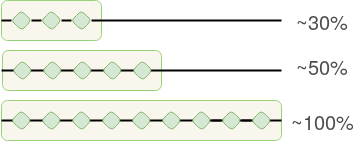
\includegraphics[width=0.5\textwidth]{imgs/workflow_reduction_2.png}
%\end{figure}
%\end{frame}
%
%\begin{frame}
%\frametitle{Workflow}
%\begin{textblock*}{5cm}(300px,10px) % {block width} (coords)
%	\includegraphics[width=50px]{imgs/wi_1.png}
%\end{textblock*}
%\framesubtitle{Trace reduction step (iii)}
%The stored information for every unique MPI call is:
%\begin{itemize}
%	\item \textbf{Number of repetitions}
%	\item \textbf{Mean time time between repetitions}
%	\item Entire call path
%	\item Previous burst performance information
%	\item Calculated delta
%	\item \textit{All timestamps}
%\end{itemize}
%\vfill
%\pause
%\begin{block}{The key point for scalability}
%	HPC applications are strongly repetitive over time so number of unique MPI calls will remain despite the increasing problem size.
%\end{block}
%\end{frame}

\begin{frame}
\frametitle{Workflow}
\begin{textblock*}{5cm}(300px,10px) % {block width} (coords)
	\includegraphics[width=50px]{imgs/wi_2.png}
\end{textblock*}
\framesubtitle{Loops identification}
\begin{mdframed}[backgroundcolor=blue!10,roundcorner=10pt,linewidth=0pt]
\textbf{Input} Set of unique MPI calls with attached information.\\
\textbf{Output} Set of sets of MPI calls $\rightarrow$ Loops
\end{mdframed}
\vfill
\pause

\begin{itemize}
	\item Need for some classification algorithm
	\pause
	\item \textbf{DBSCAN} as clustering algorithm (prefered to K-means)
	\begin{itemize}
		\item $\epsilon$ empirically set to 0.2 (in general)
		\item minPts set to 1
		\item Number of repetitions vs. Mean time between repetitions
	\end{itemize}
\pause
	\item Resulting clusters \textbf{will be considered loops}.
	\begin{itemize}
		\item Number of repetitions $\rightarrow$ Number of iterations.
		\item Mean time between repetitions $\rightarrow$ Mean iterations time.
	\end{itemize}
\end{itemize}
\end{frame}

\begin{frame}
\frametitle{Workflow}
\begin{textblock*}{5cm}(300px,10px) % {block width} (coords)
	\includegraphics[width=50px]{imgs/wi_2.png}
\end{textblock*}
\framesubtitle{Loops identification (ii)}
\begin{multicols}{2}
		\begin{pseudocode}{ }{ }
			\FOR 1 \text{ to } 50 \DO
			\BEGIN
				\FOR 1 \text{ to } 2 \DO
				\BEGIN
					MPI\_Call \\
				\END \\
				MPI\_Call\\
			\END\\
			\FOR 1 \text{ to } 100 \DO
			\BEGIN
				\FOR 1 \text{ to } 2 \DO
				\BEGIN
					\FOR 1 \text{ to } 2 \DO
					\BEGIN
						MPI\_Call \\
					\END\\
					MPI\_Call\\
				\END \\
				MPI\_Call\\
			\END
		\end{pseudocode}
	\columnbreak
	
	\columnbreak
	\pause
	\begin{figure}
		\includegraphics[width=0.5\textwidth]{imgs/clustering_ex_3.png}
	\end{figure}
\end{multicols}
\end{frame}

\begin{frame}
\frametitle{Workflow}
\begin{textblock*}{5cm}(300px,10px) % {block width} (coords)
	\includegraphics[width=50px]{imgs/wi_3.png}
\end{textblock*}
\framesubtitle{Loops merge (i)}
\begin{mdframed}[backgroundcolor=blue!10,roundcorner=10pt,linewidth=0pt]
\textbf{Input} Set of loops.\\
\textbf{Output} Set of top level loops with its related nested loops.
\end{mdframed}
\vspace{10px}
\pause
Intuition
\begin{itemize}
	\item Isolated loops are just \textbf{pieces of the overall puzzle}.
	\item By discover its hierarchical relations \textbf{the structure of the application will be betrayed}.
\end{itemize}
\pause
Some clues
\begin{itemize}
	\item Outer loop will have \textbf{less iterations} than nested one.
	\item Outer loop will spend \textbf{more time} per iteration.
	%\item Outer loop will \textbf{explain the same amount of time} as inner loop.
\end{itemize}
\end{frame}

\begin{frame}
\frametitle{Workflow}
\begin{textblock*}{5cm}(300px,10px) % {block width} (coords)
	\includegraphics[width=50px]{imgs/wi_3.png}
\end{textblock*}
\framesubtitle{Loops merge (ii)}
\begin{multicols}{2}
	\begin{figure}
		\includegraphics[width=0.3\textwidth]{imgs/clustering_ex_3_pse.png}
	\end{figure}
	\columnbreak
	\begin{figure}
		\includegraphics[width=0.4\textwidth]<1>{imgs/clustering_ex_3.png}
		\includegraphics[width=0.4\textwidth]<2->{imgs/clustering_ex_3_2.png}
	\end{figure}
\end{multicols}
\begin{itemize}
	%\item $O(\frac{n^{2}-n}{2}) \approx O(n^{2})$ comparissons
	\pause
	\item Reduce search space by classify loops by its delta
	\begin{itemize}
		\item All lies on same $f(x)=\frac{\delta*T_{exe}}{x}$ being $0 < \delta < 1$
	\end{itemize}
	\item And then merge them in a less to more iterations fashion
\end{itemize}
\pause
\begin{block}{Keynote}
	This mechanism is then used for phases detection as well.
\end{block}
\end{frame}

\begin{frame}
\begin{textblock*}{5cm}(300px,10px) % {block width} (coords)
	\includegraphics[width=50px]{imgs/wi_4.png}
\end{textblock*}
\frametitle{Workflow}
\framesubtitle{Pseudocode construction (i)}
\begin{mdframed}[backgroundcolor=blue!10,roundcorner=10pt,linewidth=0pt]
\textbf{Input} Set of top level loops with rank conditional structures.\\
\textbf{Output} Pseudocode representing the actual application structure.
\end{mdframed}
\vfill
\pause
\begin{itemize}
	\item Straightforward construction
	\item Just a refination of the data is needed
	\begin{enumerate}
		\item Extracting common call path levels from code block (loops and conditional blocks)
		\item Removing \textbf{contiguous repetitive information} what has not been removed in previous step
	\end{enumerate}
\end{itemize}
\end{frame}

%\begin{frame}
%	\begin{textblock*}{5cm}(300px,10px) % {block width} (coords)
%		\includegraphics[width=50px]{imgs/wi_4.png}
%	\end{textblock*}
%	\frametitle{Workflow}
%	\framesubtitle{Pseudocode construction (ii)}
%	\begin{multicols}{3}
%		\begin{figure}
%			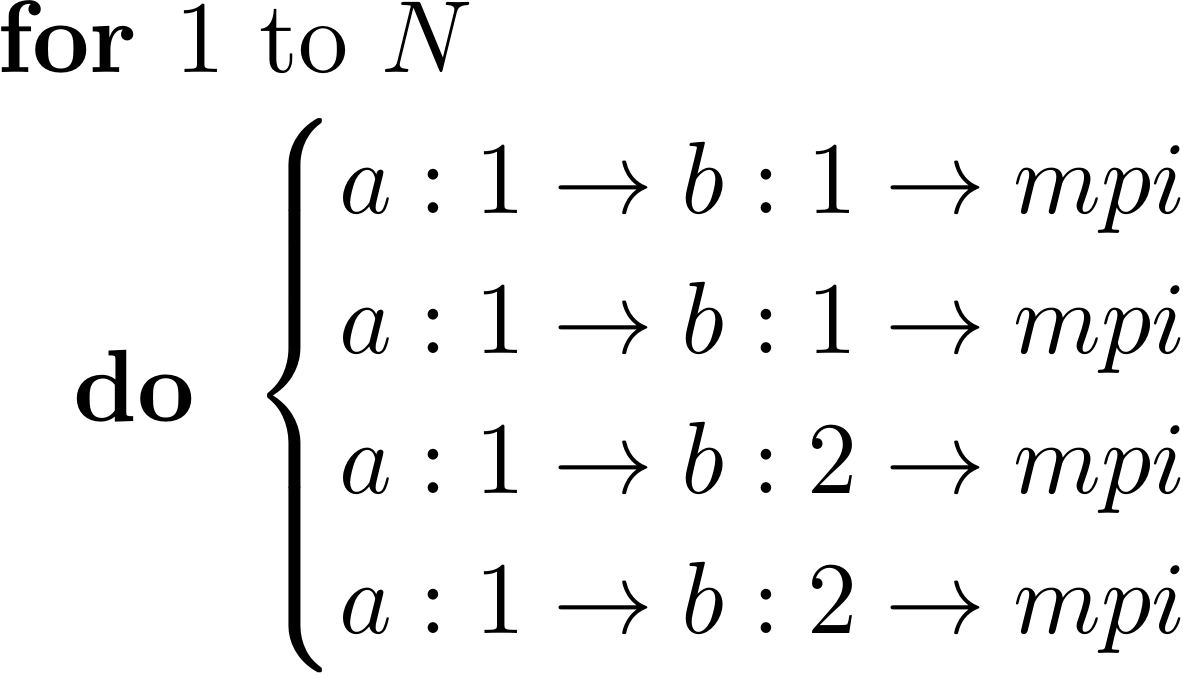
\includegraphics[width=0.3\textwidth]{imgs/workflow_pseudocode_1.png}
%			%\caption{Raw pseudocode}
%		\end{figure}
%		\columnbreak
%		\pause
%		\begin{figure}
%			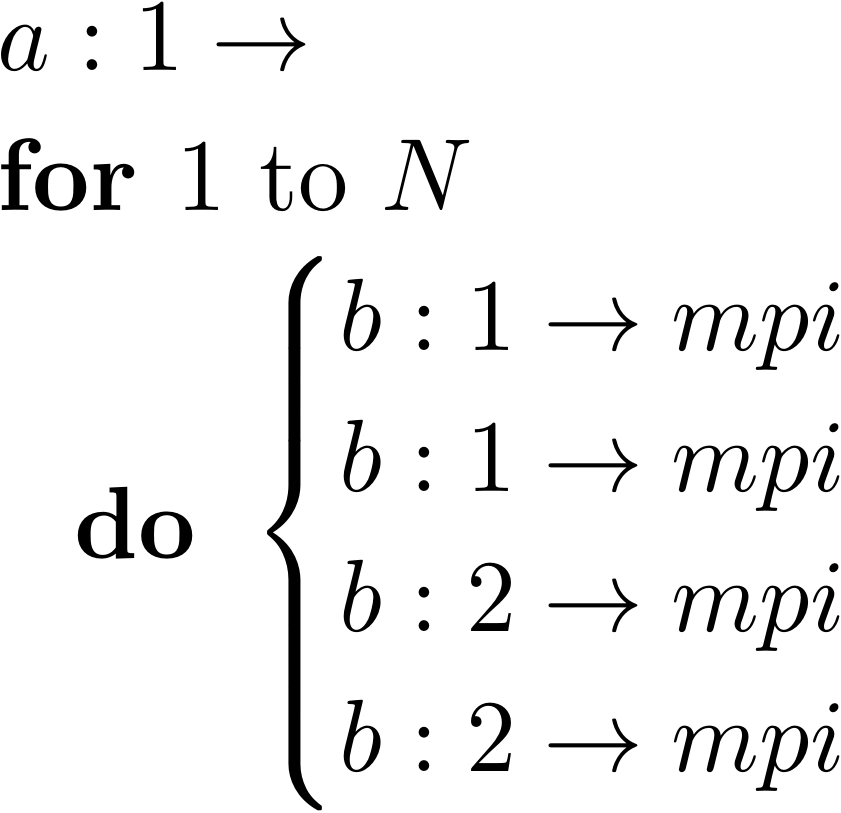
\includegraphics[width=0.18\textwidth]{imgs/workflow_pseudocode_2.png}
%			%\caption{After extract common call path}	
%		\end{figure}
%		\columnbreak
%		\pause
%		\begin{figure}
%			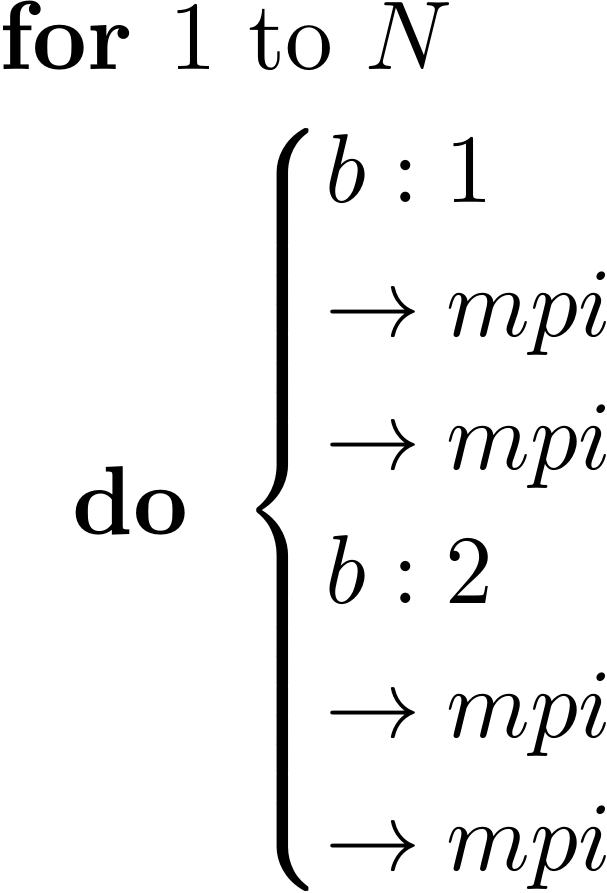
\includegraphics[width=0.14\textwidth]{imgs/workflow_pseudocode_3.png}
%			%\caption{After extract contiguous call path}
%		\end{figure}
%		\columnbreak
%	\end{multicols}
%\end{frame}

\begin{frame}
\begin{textblock*}{5cm}(300px,10px) % {block width} (coords)
	\includegraphics[width=50px]{imgs/wi_4.png}
\end{textblock*}
\frametitle{Workflow}
\framesubtitle{Pseudocode construction (ii)}
\begin{figure}
	\includegraphics[width=0.8\textwidth]{imgs/example_output_1.png}
	%\caption{Example console output}
\end{figure}
\pause
\begin{figure}
	\includegraphics[width=0.8\textwidth]{imgs/interactive_shell_example.png}
\end{figure}
\end{frame}

\section{Best features analysis}
\begin{frame}
\frametitle{Best features analysis}
Some problems have been detected like cluster aliasing/split
\begin{itemize}
	\item Solved by timestamps analysis
\end{itemize}
\textbf{Validate} our first intutition \\
\textbf{Explore} the possibility to find out...\\
\begin{itemize}
	\item \textbf{Alternative features} for classification
	\item \textbf{Additional features} for classification
	\begin{itemize}
		\item \#Instructions, \#Cycles, \#Loads, \#(Cond, Uncond, Total) branches. \#FP instructions\footnote{Strictly limited by available hardaware}
	\end{itemize}
\end{itemize}
\pause
Two steps:
\begin{enumerate}
	\item Data acquisition \& post-process
	\begin{itemize}
		\item Extrae just can monitorize calls to shared libraries
		\item Loops monitors injection by \textbf{Mercurium}
	\end{itemize}
	\item Analyze results and conclusion
	\begin{itemize}
		\item Principal components analysis
		\item Variable Importance by Random Forest technique
	\end{itemize}
\end{enumerate}
\end{frame}

\begin{frame}
\frametitle{Best features analysis}
\framesubtitle{Analysis of results: \textbf{Variable Importance}}
\begin{block}{Results}
	The first intuition \textbf{has been validated}!\\
	But alternative/additional features have not been found $\rightarrow$ Future work
\end{block}
\begin{figure}
	\includegraphics[height=0.7\textheight]{imgs/varimp_results.png}
\end{figure}
\end{frame}

\section{Results}
\subsection{Lulesh 2.0}
\begin{frame}
	\frametitle{Results}
	\framesubtitle{Lulesh 2.0}
	\begin{multicols*}{2}
	\begin{mdframed}[backgroundcolor=blue!10,roundcorner=10pt,linewidth=0pt]
	Execution:
	\begin{itemize}
		\item 6014 code lines
		\item 128 parallel processes
		%\item 30 iterations
		\item $\approx160MB$ tracefile
	\end{itemize}
	Analysis:
	\begin{itemize}
		\item Filter all $\delta < 10\%$\\
		\item CPU burst $time > 6ms$
	\end{itemize}
	\end{mdframed}
	\pause
	Results:
	\begin{itemize}
		\item 30 iterations loop
		\item 5 long CPU burst above 6ms
		\item 1 Data conditioned MPI call
		\item 56 no conditioned MPI calls
	\end{itemize}
	\columnbreak
	%\begin{figure}
	%	\includegraphics[height=0.3\textheight]{imgs/clustering_val_10.png}
	%\end{figure}
	\begin{figure}
		\includegraphics[height=0.8\textheight]{imgs/result_val_10.png}
	\end{figure}
	\end{multicols*}
\end{frame}

\begin{frame}
\frametitle{Results}
\framesubtitle{Lulesh 2.0 (i)}
\begin{figure}
	\includegraphics[width=0.8\textwidth]<1>{imgs/lulesh_trace_1.png}
	\includegraphics[width=0.8\textwidth]<2>{imgs/lulesh_trace_1_cnt.png}
	\caption{Lulesh 2.0 128 MPI ranks -- 30 iterations}
\end{figure}
\end{frame}

\begin{frame}
	\frametitle{Results}
	\framesubtitle{Lulesh 2.0 (ii)}
	\begin{figure}
		\includegraphics[height=0.3\textheight]{imgs/result_val_10_bursts.png}
	\end{figure}
	\begin{figure}
		\includegraphics[height=0.4\textheight]{imgs/lulesh_trace_3.png}
	\end{figure}
\end{frame}

\begin{frame}
	\frametitle{Results}
	\framesubtitle{Lulesh 2.0 (iii)}
	\begin{figure}
		\includegraphics[height=0.3\textheight]<1>{imgs/lulesh_comm_phase_1.png}
		\includegraphics[height=0.3\textheight]<2>{imgs/lulesh_comm_phase_2.png}
		%\includegraphics[height=0.3\textheight]<3>{imgs/lulesh_comm_phase_3.png}
		%\includegraphics[height=0.3\textheight]<4>{imgs/lulesh_comm_phase_4_5.png}
	\end{figure}

	\begin{table}[height=0.1\textheight]
		\centering
		\caption{Total MPI calls}
		\resizebox{0.5\textwidth}{!}{%
		\begin{tabular}{@{}l|llllll@{}}
			\toprule
			& MPI\_Isend & MPI\_Irecv & MPI\_Wait & MPI\_Waitall & MPI\_Allreduce & MPI\_Comm\_rank \\ \midrule
			Rank 0 & 300        & 510        & 510       & 90           & 29             & 270             \\ \bottomrule
		\end{tabular}%
	}
	\end{table}

	\begin{table}[height=0.2\textheight]
		\centering
		\caption{MPI calls countes by communication phases}
		\label{my-label}
		\resizebox{0.5\textwidth}{!}{%
		\begin{tabular}{@{}l|llllll@{}}
			\toprule
			& MPI\_Isend & MPI\_Irecv & MPI\_Wait & MPI\_Waitall & MPI\_Allreduce & MPI\_Comm\_rank \\ \midrule
			Comm phase 1 & 0          & 7          & 0         & 0            & 1              & 1               \\
			Comm phase 2 & 7          & 7          & 7         & 1            & 0              & 3               \\
			Comm phase 3 & 0          & 0          & 7         & 1            & 0              & 2               \\
			Comm phase 4 & 0          & 3          & 0         & 0            & 0              & 1               \\
			Comm phase 5 & 3          & 0          & 3         & 1            & 0              & 2               \\ \bottomrule
		\end{tabular}%
	}
	\end{table}
\end{frame}

\subsection{CG}
\begin{frame}
\frametitle{Results}
\framesubtitle{CG Class A}
\begin{multicols*}{2}
	\begin{mdframed}[backgroundcolor=blue!10,roundcorner=10pt,linewidth=0pt]
		Execution:
		\begin{itemize}
			\item ~2000 code lines
			\item 32 parallel processes
			\item $\approx150MB$ tracefile
		\end{itemize}
		Analysis:
		\begin{itemize}
			\item Filter all $\delta < 10\%$\\
			\item CPU burst $time > 100us$
		\end{itemize}
	\end{mdframed}
	\pause
	Results:
	\begin{itemize}
		\item 15 iterations loop
		\item 25 iterations subloop
		\item Other 3 iterations subloops
		\item 2 long CPU burst above 500us
%		\item 1 Data conditioned MPI call
%		\item 56 no conditioned MPI calls
	\end{itemize}
	\columnbreak
%	\begin{figure}
%		\includegraphics[height=0.3\textheight]{imgs/cg_32_clustering.png}
%	\end{figure}
	\begin{figure}
		\includegraphics[height=0.7\textheight]{imgs/cg_32_result.png}
	\end{figure}
\end{multicols*}
\end{frame}

\begin{frame}
\frametitle{CG (ii)}
	\begin{figure}
		\includegraphics[height=0.2\textheight]{imgs/cg_32_validation_1.png}
	\end{figure}
	\pause
	\begin{figure}
		\includegraphics[height=0.2\textheight]{imgs/cg_32_validation_2.png}
	\end{figure}
	\pause
	\begin{figure}
		\includegraphics[height=0.2\textheight]{imgs/cg_32_validation_3.png}
	\end{figure}
\end{frame}

\section{Scalability}
\begin{frame}
	\frametitle{Scalability}
	\begin{multicols}{2}
	\begin{figure}
		\includegraphics[height=0.2\textheight]{imgs/plots/cg_a_bd.png}
	\end{figure}
	\begin{figure}
		\includegraphics[height=0.2\textheight]{imgs/plots/cg_b_bd.png}
	\end{figure}
	\begin{figure}
		\includegraphics[height=0.2\textheight]{imgs/plots/cg_c_bd.png}
	\end{figure}
	\columnbreak
	\begin{figure}
		\includegraphics[height=0.2\textheight]{imgs/plots/cg_a_sp.png}
	\end{figure}
	\begin{figure}
		\includegraphics[height=0.2\textheight]{imgs/plots/cg_b_sp.png}
	\end{figure}
	\begin{figure}
		\includegraphics[height=0.2\textheight]{imgs/plots/cg_c_sp.png}
	\end{figure}
	\end{multicols}
\end{frame}

\begin{frame}
	\frametitle{Scalability}
	
	\begin{figure}
		\includegraphics[width=0.5\textwidth]{imgs/plots/cg_red_and_trace.png}
	\end{figure}
\end{frame}

\section{Conclusions}
\begin{frame}
\frametitle{Conclusions}
\begin{itemize}[<+->]
	\item New approach has been explored.
	\item That demonstrates how works reasonably well.
	\item Iterations mean time and number of iterations demonstrates to be valuable features for classification
	\item With general linear complexity with trace size.
\end{itemize}
\end{frame}

\section{Future work}
\begin{frame}
	\frametitle{Future work}
	\begin{itemize}[<+->]
		\item Improve Reduce phase times by, e.g. Parallelize the reduction using for example well-known infrastructures like Hadoop.
		\item More research for select the best features set that avoids cluster aliasing/split.
		\item Explore the alternative to merge different ranks mpi calls at Trace reduce step.
		\item Exploring the possibility to use sampling techniques to get more detailed view of the structure of an application.
		
	\end{itemize}
\end{frame}

\begin{frame}
\titlepage
\end{frame}


%==================================================
%==================================================
%==================================================
%==================================================

\appendix

\begin{frame}
\frametitle{Refinement}
Even if it \textbf{works pretty well} in general. \\
Some problems \textbf{have been identified}.
\begin{enumerate}
	\item \textbf{Cluster aliasing} when two different loops behaves similarly enough over our defined space
	\item \textbf{Hidden superloop} when not detected superloop prevents from a good structure detection.
	\item \textbf{Cluster split} when MPI calls belonging to the same loop behaves in a different way.
\end{enumerate}
All three \textbf{have been solved by looking to timestamps}.

\end{frame}

\begin{frame}
	\frametitle{Proposal modifications (ii)}
	\framesubtitle{Cluster aliasing}
	\begin{block}{Keynote}
		Aliasing can be detected and solved \textbf{looking at timestamps}.
	\end{block}
	\begin{multicols}{2}
	\begin{figure}
		\includegraphics[height=0.3\textheight]{imgs/aliasing_example_pse.png}
	\end{figure}
	\columnbreak
	\begin{figure}
		\includegraphics[width=0.3\textwidth]{imgs/aliasing_ex_clustering.png}
	\end{figure}
	\end{multicols}
	\pause
	\begin{multicols}{2}
		\null \vfill
		\begin{table}[]
			\centering
			\begin{tabular}{l|ll}
				MPI\_A & 1 & 3 \\
				MPI\_B & 2 & 4 \\
				MPI\_C & 5 & 7 \\
				MPI\_D & 6 & 8
			\end{tabular}
		\end{table}
		\vfill \null
		\columnbreak
		\pause
		\null \vfill
		\begin{table}[]
			\centering
			\begin{tabular}{l|llll}
				MPI\_A & 1 & 3 &   &   \\
				MPI\_B & 2 & 4 &   &   \\ \hline
				MPI\_C &   &   & 5 & 7 \\
				MPI\_D &   &   & 6 & 8
			\end{tabular}
		\end{table}
		\vfill \null
	\end{multicols}
\end{frame}

\begin{frame}
	\frametitle{Proposal modifications}
	\framesubtitle{Hidden superloop}
	\begin{block}{Keynote}
		Similarly than with aliasing, \textbf{looking at timestamps}.
	\end{block}
	\begin{multicols}{2}
		\begin{figure}
			\includegraphics[height=0.2\textheight]{imgs/hidden_superloon_ex_pse.png}
		\end{figure}
		\columnbreak
		\begin{figure}
			\includegraphics[width=0.3\textwidth]{imgs/hidden_superloop_ex_clustering.png}
		\end{figure}
	\end{multicols}
	\pause
	\begin{multicols}{2}
		\begin{table}[]
			\begin{tabular}{l | llll}
				MPI\_A & 1 & 2 & 5 & 6 \\ 
				MPI\_B & 3 & 4 & 7 & 8
			\end{tabular}
		\end{table}
		\pause
		\columnbreak
		\begin{table}[]
		\begin{tabular}{l | llllllll}
			MPI\_A & 1 & 2 &   &   & 5 & 6 &   &   \\ \hline
			MPI\_B &   &   & 3 & 4 &   &   & 7 & 8
		\end{tabular}
		\end{table}
	\end{multicols}
\end{frame}

\begin{frame}
\frametitle{Proposal modifications}
\framesubtitle{Cluster split}

\begin{multicols}{2}
	\begin{figure}
		\includegraphics[height=60px]{imgs/split_example_2.png}
	\end{figure}
%	\begin{pseudocode}{ }{ }
%		\FOR i=1 \text{ to } 10 \DO
%		\BEGIN
%		MPI\_B()\\
%		\IF isPair(i) \THEN
%			MPI\_A()\\
%		MPI\_B()\\
%		\END
%	\end{pseudocode}
	\columnbreak
	\begin{figure}
		\includegraphics[width=0.3\textwidth]<1>{imgs/clustering_val_8_1.png}
		\includegraphics[width=0.3\textwidth]<2->{imgs/clustering_val_8.png}
	\end{figure}
\end{multicols}
\pause
Whether MPI call is conditioned
\begin{itemize}
	\item \#repetitions and mean time bw. reps. change (in same proportion).
\end{itemize} 
\pause
By ``reverse loop merging'' and times checking
\begin{figure}
	\includegraphics[height=0.3\textheight]{imgs/result_val_9.png}
\end{figure}
\end{frame}

\begin{frame}
\frametitle{Data analysis}
\framesubtitle{Data acquisition (i)}
Desired data...\\
\begin{itemize}
\item PCA\footnote{Principal component analysis}: Set of observations with set of features, i.e. Set of loops with with \textbf{iteration-level aggregated features}. 
\item Variable Importance Same data as in production traces but labeled, i.e. textbf{With information to what loop every MPI call belongs to}.
\end{itemize}
How to obtain it\\
\begin{enumerate}
\item The needed information is not in trace so ...
\item \textbf{Manually inject monitors} to the source code
\begin{itemize}
	\item Very tough and error prone for huge source codes
\end{itemize}
\item Alternatively use source-to-source compiler to \textbf{do it utomaticaly}
\begin{itemize}
	\item Mercurium
\end{itemize}
\end{enumerate}
\end{frame}

\begin{frame}
\frametitle{Data analysis}
\framesubtitle{Data acquisition (i)}
\begin{figure}
\includegraphics[width=0.7\textwidth]{imgs/mercurium_internals.png}
\caption{Mercurium internals overview}
\end{figure}
\end{frame}

\begin{frame}
\frametitle{Data analysis}
\framesubtitle{Data acquisition (ii)}
\begin{multicols}{2}
\begin{pseudocode}{PCA}{ }
MLoopInit(loop_{line}, loop_{file})\\
\FOR i \in I \DO
\BEGIN
MIterInit(chance)\\
...\\
MIterFini()\\
\END\\
MLoopFini()		
\end{pseudocode}
\begin{itemize}
\item MLoopInit and MLoopFini fire loops boundaries
\item MIterInit and MiterFini fire iteration boundaries with hwc information o trace
\end{itemize}
\columnbreak
\pause
\begin{pseudocode}{VarImp}{ }
MLoopInit(loop_{line}, loop_{file})\\
\FOR i \in I \DO
\BEGIN
...\\
MBefCall()\\
MPI\_Call()\\
MPIAftCall()\\
...\\
\END\\
MLoopFini()		
\end{pseudocode}
\begin{itemize}
\item MLoopInit and MLoopFini keep track entry/exit loops
\item MPIBefCall and MPIAftCall fire loop id
\end{itemize}
\end{multicols}
\end{frame}

\begin{frame}
\frametitle{Data analysis}
\framesubtitle{Analysis of results (i): \textbf{PCA}}
\begin{figure}
	\includegraphics[height=0.9\textheight]{imgs/pcas_results.png}
\end{figure}
\end{frame}

%\bibliography{bibliography}
%\bibliographystyle{apalike}

\end{document}